% !TEX program = xelatex

\documentclass[12pt, a4paper]{article}

\usepackage{fontspec}
\setmainfont[Ligatures=TeX]{Linux Libertine O}

\usepackage[hidelinks, colorlinks = true, urlcolor = blue]{hyperref}
\usepackage{indentfirst}
\usepackage{graphicx}
\usepackage[left=2cm,right=2cm,top=2.5cm,bottom=2.5cm]{geometry}
\usepackage{lipsum}

\begin{document}

\begin{titlepage}

\begin{figure}[h!]
  \begin{center}
    
\includegraphics[width=3cm]{assets/auth.pdf}
    \label{fig:cover_auth_logo}
  \end{center}
\end{figure}

\centering
\Large Αριστοτέλειο Πανεπιστήμιο Θεσσαλονίκης\\
\Large Πολυτεχνική Σχολή\\
%\large Τμήμα Ηλεκτρολόγων Μηχανικών και Μηχανικών Υπολογιστών\\
%\large Τομέας Τηλεπικοινωνιών

\vspace{\fill}

\LARGE \textbf{Java socket programming} \\
\LARGE \textbf{Δίκτυα 2}

\vspace{\fill}

\Large Θεόδωρος Κατζάλης \\
\Large ΑΕΜ:9282 \\ 
\Large katzalis@auth.gr

\vspace{\fill}
\raggedright

\centering
\vspace{\fill}
\today

\end{titlepage}

%\maketitle


\pagebreak
\tableofcontents
%\pagebreak

% \section{Lorem}
% \lipsum


\vspace{3cm}

\section{Image}
Αξίζει να σημειωθεί, μιας και δεν φαίνεται στα wireshark captures, ότι είχαμε δημιουργήσει ένα custom filter: \textbf{host 155.207.18.208 and udp} το οποίο το επιλέγαμε προτού αρχίσουμε το capturing των πακέτων.

%\vspace{3cm}

\begin{figure}[h!]
\centering
	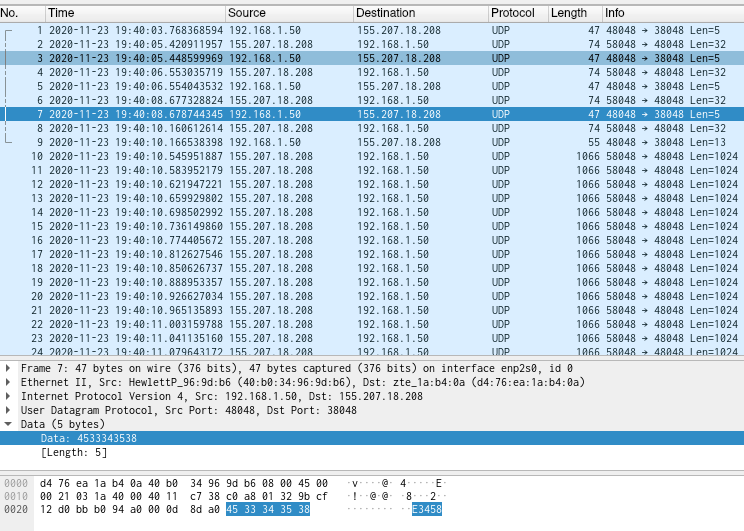
\includegraphics[height=.4\textheight, width=\textwidth, keepaspectratio]{assets/wireshark/image1.png}
	\caption{Echo request code} 
\end{figure}

\pagebreak
\begin{figure}[h!]
\centering
	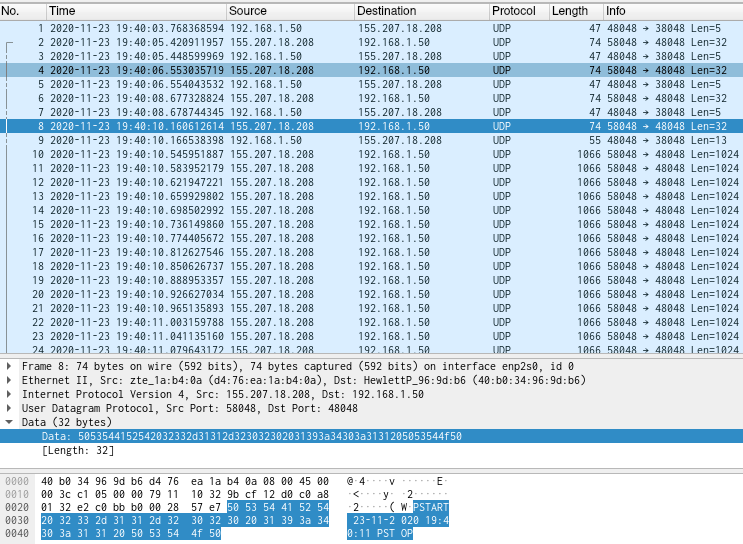
\includegraphics[height=.4\textheight, width=\textwidth, keepaspectratio]{assets/wireshark/image2.png}
	\caption{Echo response time} 
\end{figure}

\begin{figure}[h!]
\centering
	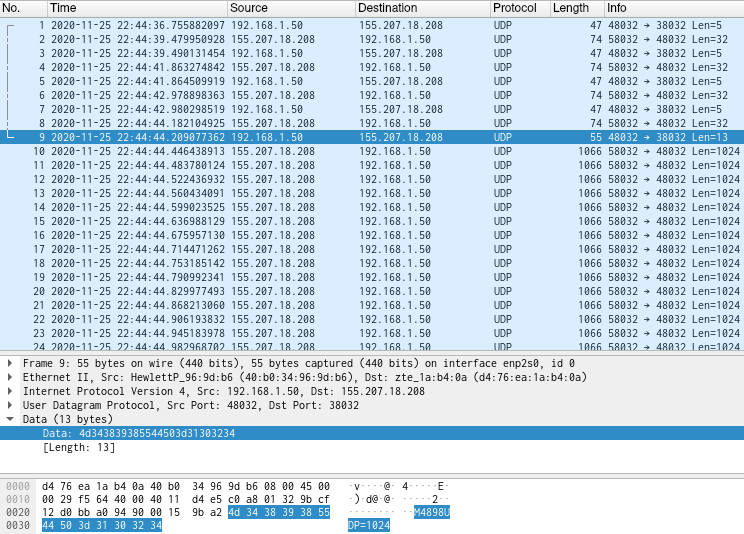
\includegraphics[height=.4\textheight, width=\textwidth, keepaspectratio]{assets/wireshark/image3.png}
	\caption{Image request code} 
\end{figure}


\pagebreak
\begin{figure}[h!]
\centering
	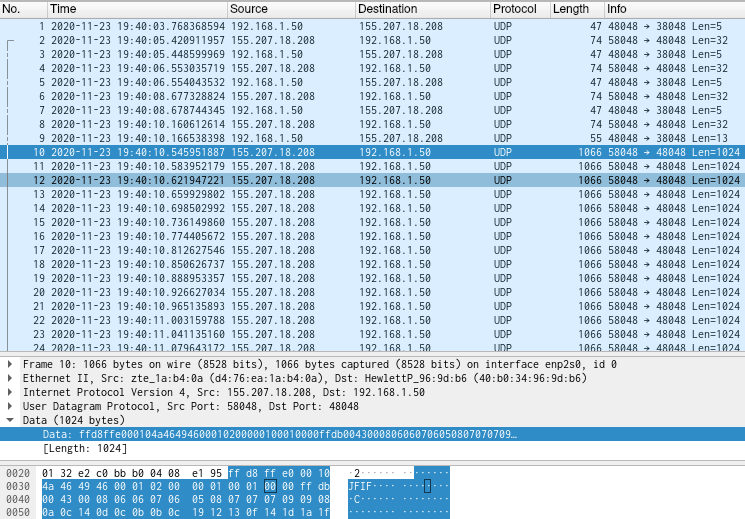
\includegraphics[height=.4\textheight, width=\textwidth, keepaspectratio]{assets/wireshark/image4.png}
	\caption{Image response data} 
\end{figure}


\section{Audio}

\begin{figure}[h!]
\centering
	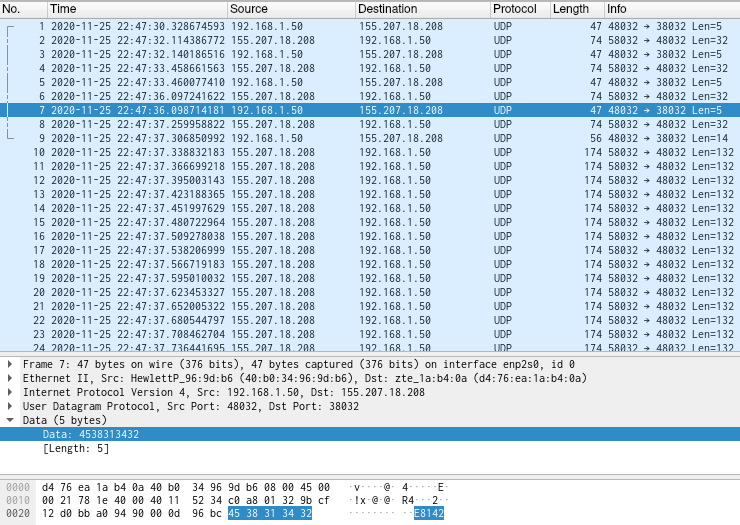
\includegraphics[height=.4\textheight, width=\textwidth, keepaspectratio]{assets/wireshark/audio1.png}
	\caption{Echo request code} 
\end{figure}

\pagebreak
\begin{figure}[h!]
\centering
	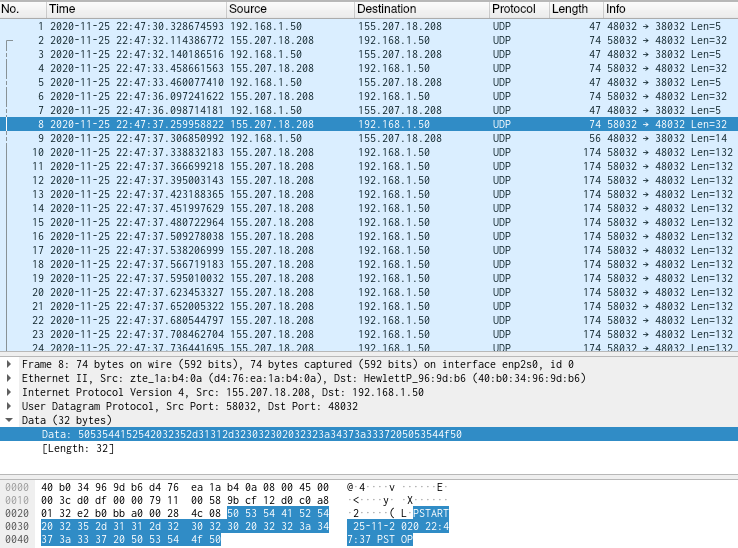
\includegraphics[height=.4\textheight, width=\textwidth, keepaspectratio]{assets/wireshark/audio2.png}
	\caption{Echo response time} 
\end{figure}

\begin{figure}[h!]
\centering
	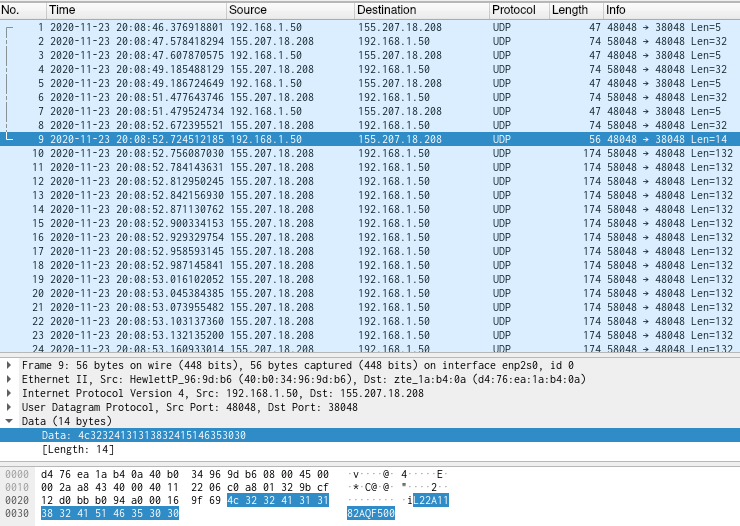
\includegraphics[height=.4\textheight, width=\textwidth, keepaspectratio]{assets/wireshark/audio3.png}
	\caption{Audio request code} 
\end{figure}

\pagebreak
\begin{figure}[h!]
\centering
	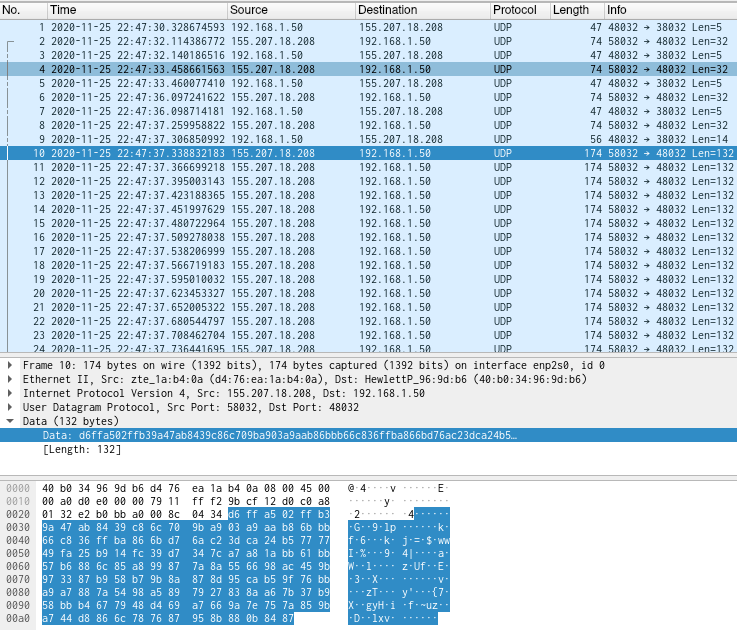
\includegraphics[height=.4\textheight, width=\textwidth, keepaspectratio]{assets/wireshark/audio4.png}
	\caption{Audio response data} 
\end{figure}


\section{Ithakicopter TCP version}

\begin{figure}[h!]
\centering
	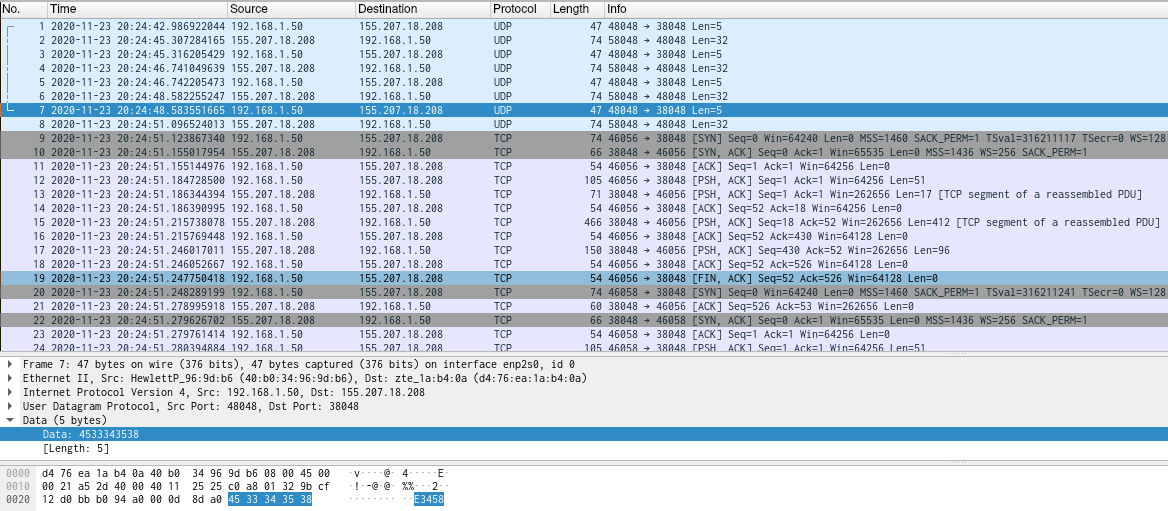
\includegraphics[height=.4\textheight, width=\textwidth, keepaspectratio]{assets/wireshark/copter1.png}
	\caption{Echo request code} 
\end{figure}

\pagebreak
\begin{figure}[h!]
\centering
	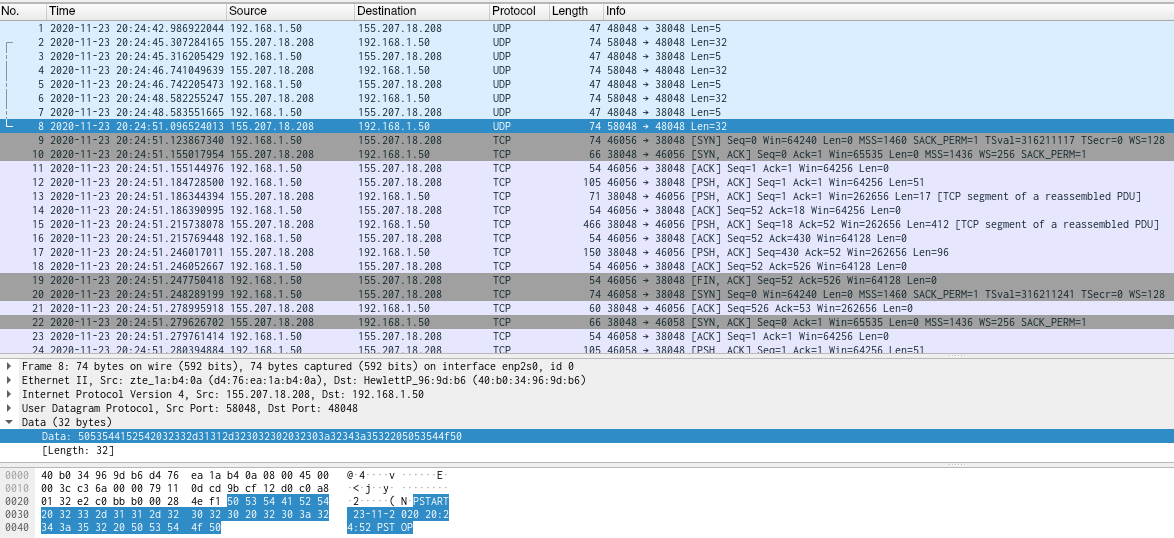
\includegraphics[height=.4\textheight, width=\textwidth, keepaspectratio]{assets/wireshark/copter2.png}
	\caption{Echo response time} 
\end{figure}

\begin{figure}[h!]
\centering
	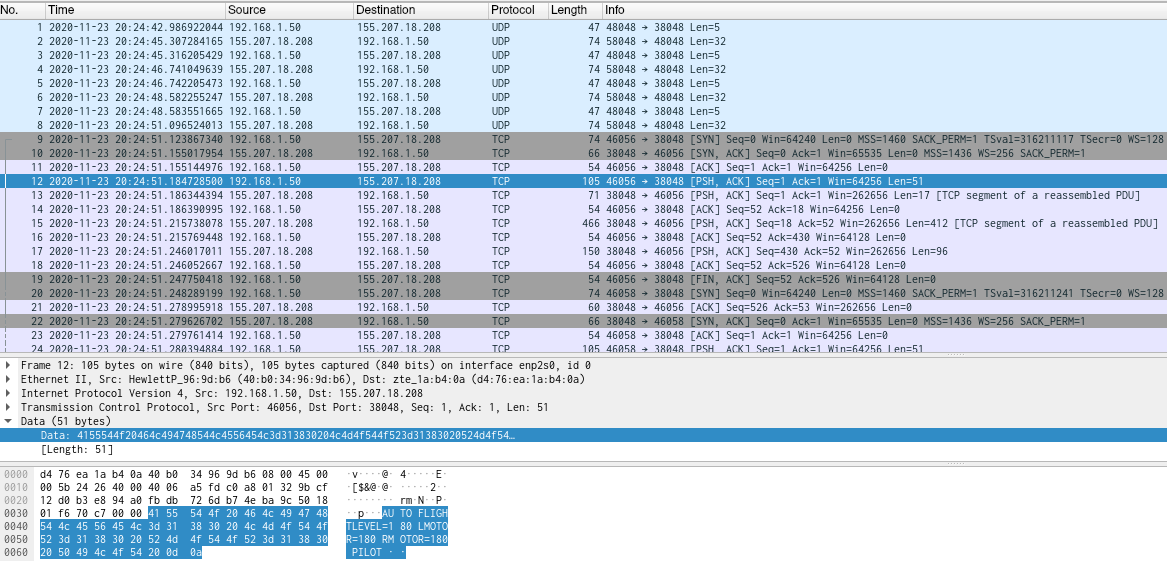
\includegraphics[height=.4\textheight, width=\textwidth, keepaspectratio]{assets/wireshark/copter3.png}
	\caption{Copter output stream} 
\end{figure}

\pagebreak

\begin{figure}[h!]
\centering
	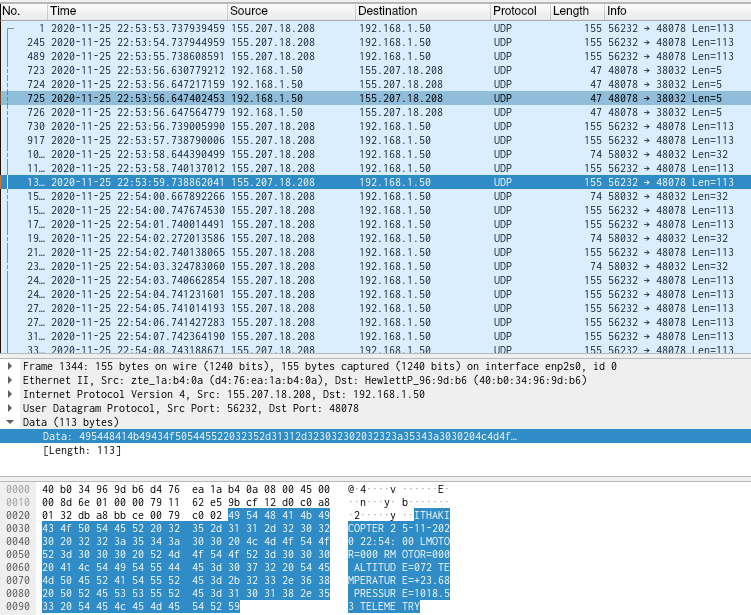
\includegraphics[height=.4\textheight, width=\textwidth, keepaspectratio]{assets/wireshark/copter4.png}
	\caption{Copter input stream} 
\end{figure}

\section{Car fault diagnostics}

\begin{figure}[h!]
\centering
	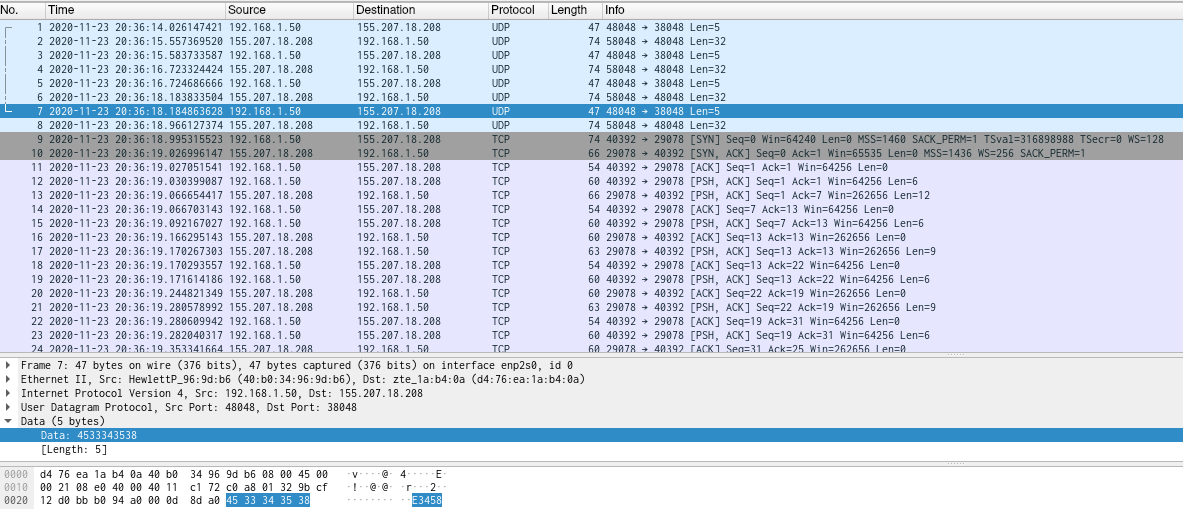
\includegraphics[height=.4\textheight, width=\textwidth, keepaspectratio]{assets/wireshark/vehicle1.png}
	\caption{Echo request code} 
\end{figure}

\pagebreak
\begin{figure}[h!]
\centering
	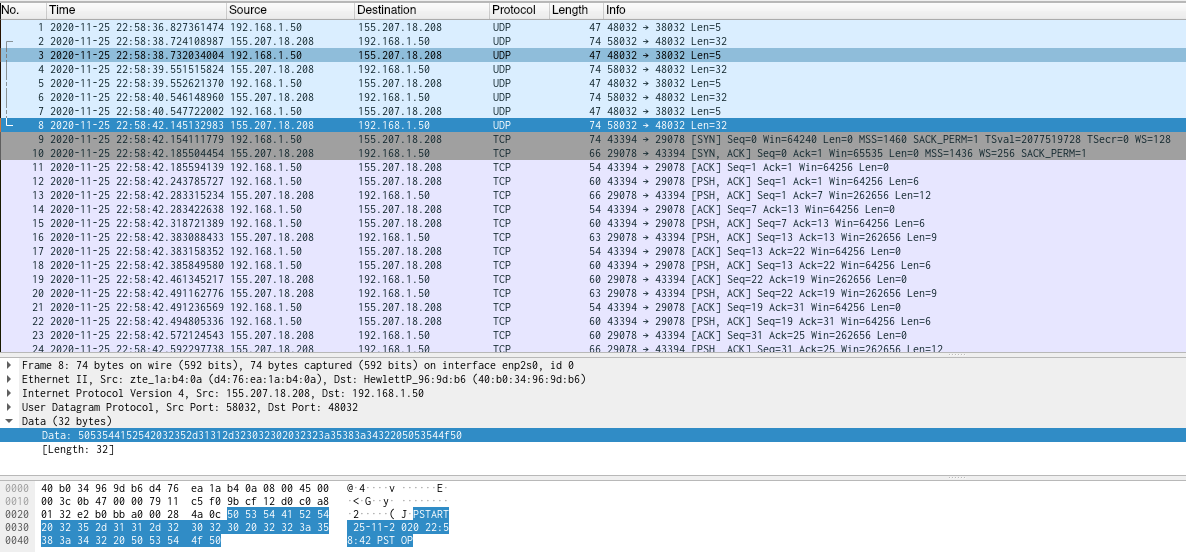
\includegraphics[height=.4\textheight, width=\textwidth, keepaspectratio]{assets/wireshark/vehicle2.png}
	\caption{Echo response time} 
\end{figure}

\begin{figure}[h!]
\centering
	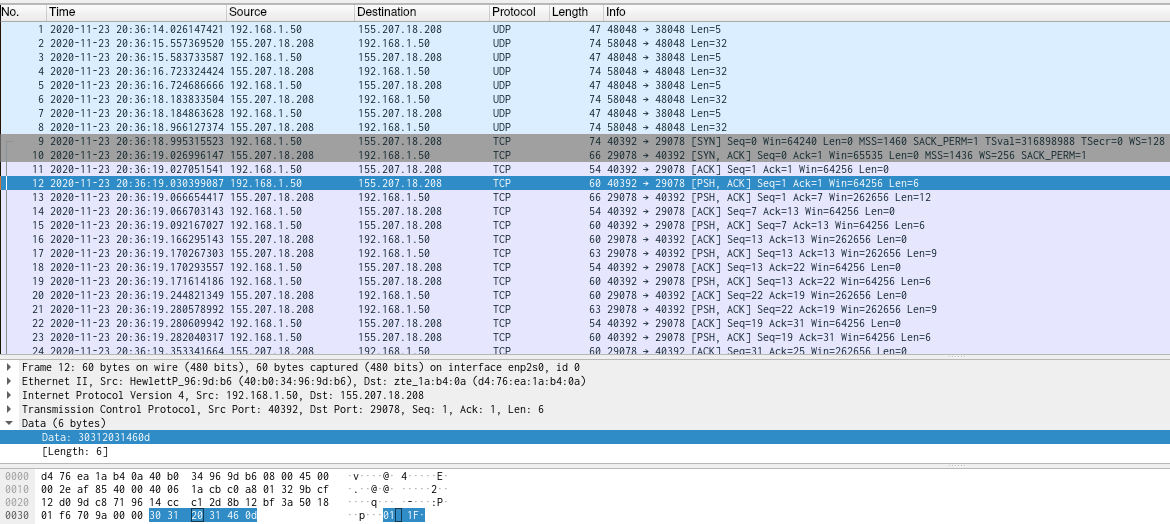
\includegraphics[height=.4\textheight, width=\textwidth, keepaspectratio]{assets/wireshark/vehicle3.png}
	\caption{Vehicle output stream} 
\end{figure}

\pagebreak

\begin{figure}[h!]
\centering
	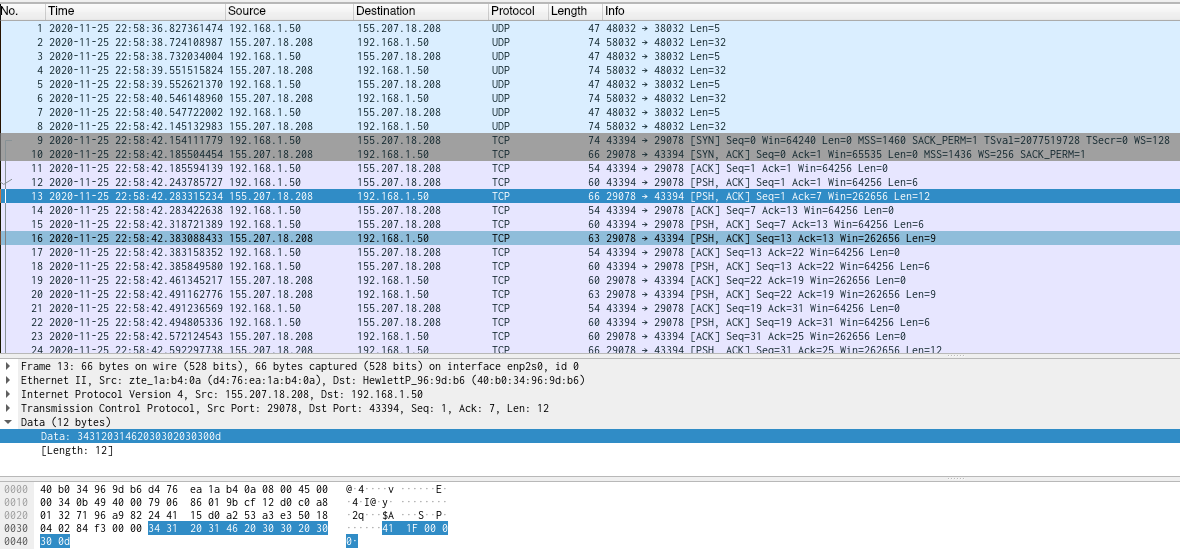
\includegraphics[height=.4\textheight, width=\textwidth, keepaspectratio]{assets/wireshark/vehicle4.png}
	\caption{Vehicle input stream} 
\end{figure}

\end{document}
